
%(BEGIN_QUESTION)
% Copyright 2011, Tony R. Kuphaldt, released under the Creative Commons Attribution License (v 1.0)
% This means you may do almost anything with this work of mine, so long as you give me proper credit

This Allen-Bradley MicroLogix 1100 PLC ``schedules'' a setpoint value for a heat-treat furnace temperature control system.  The setpoint value is selected by the first sequencer instruction (SQO) from multiple PLC memory registers and placed in memory register N7:10 where it will be read by another portion of the program to be interpreted as the desired temperature of the furnace.  The second sequencer instruction (SQO) allows for different time intervals at each setpoint value in the schedule.  The purpose of this sequencing program is to select different furnace temperature setpoint values at different times, in order to properly heat-treat samples of alloyed metal placed in the furnace:

$$\includegraphics[width=15.5cm]{i04658x01.eps}$$

\filbreak

$$\includegraphics[width=15.5cm]{i04658x02.eps}$$

Identify the proper number values to store in the appropriate {\tt N7} registers to generate the following schedule, assuming 1-degree Fahrenheit resolution for the integer temperature setpoint values (e.g. an integer value of ``562'' means 562 degrees Fahrenheit):

\begin{itemize}
\item{} 750 degrees for 10 minutes
\item{} 1050 degrees for 35 minutes
\item{} 500 degrees for 20 minutes
\item{} 0 degrees (indefinite cool-down period) 
\end{itemize}

Also, identify the ``normal'' pushbutton switch contact statuses (NO vs. NC) for the ``Start'' and ``Stop'' pushbuttons controlling this temperature sequencing program, and how this program might be edited to provide a ``reset'' pushbutton control to return back to step 1 of the heating schedule.

\vskip 20pt \vbox{\hrule \hbox{\strut \vrule{} {\bf Suggestions for Socratic discussion} \vrule} \hrule}

\begin{itemize}
\item{} Identify the purpose of the rung with the {\tt B3:2/0} coil at the end.
\end{itemize}

\underbar{file i04658}
%(END_QUESTION)





%(BEGIN_ANSWER)

% No blank lines allowed between lines of an \halign structure!
% I use comments (%) instead, so that TeX doesn't choke.

$$\vbox{\offinterlineskip
\halign{\strut
\vrule \quad\hfil # \ \hfil & 
\vrule \quad\hfil # \ \hfil \vrule \cr
\noalign{\hrule}
%
% First row
{\bf Register} & {\bf Value} \cr
%
\noalign{\hrule}
%
% Another row
N7:1 & 750 \cr
%
\noalign{\hrule}
%
% Another row
N7:2 & 1050 \cr
%
\noalign{\hrule}
%
% Another row
N7:3 & 500 \cr
%
\noalign{\hrule}
%
% Another row
N7:4 & 0 \cr
%
\noalign{\hrule}
%
% Another row
N7:6 & 600 \cr
%
\noalign{\hrule}
%
% Another row
N7:7 & 2100 \cr
%
\noalign{\hrule}
%
% Another row
N7:8 & 1200 \cr
%
\noalign{\hrule}
%
% Another row
N7:9 & 0 \cr
%
\noalign{\hrule}
} % End of \halign 
}$$ % End of \vbox


%(END_ANSWER)





%(BEGIN_NOTES)

Both the ``Start'' and ``Stop'' pushbutton switches need to have normally-open (NO) contacts.  A ``return to step 1'' input could energize a pair of reset coils (RES) addressed to each of the two sequencer addresses.

%INDEX% PLC, ladder logic program analysis and explanation (Allen-Bradley MicroLogix 1100)

%(END_NOTES)


